\documentclass[11pt]{article}
\usepackage[margin=1in, left=1.2in]{geometry}

\usepackage[dvipsnames]{xcolor}
\newcommand{\rev}[1]{{\color{RoyalBlue}#1}}


% use proper unicode fonts
\usepackage[T1]{fontenc}
\usepackage[utf8]{inputenc}

\usepackage{amsmath} % for better display of equations
\usepackage{natbib} 


\usepackage{graphicx}
%\usepackage[nomarkers,nolists,heads]{endfloat}
\usepackage{caption}
\DeclareCaptionLabelFormat{appendix}{#1 S#2}
\captionsetup{labelformat=appendix}


% Tikz libraries for building the diagram
\usepackage{tikz}
\usepackage{tikz-cd}
\usetikzlibrary{calc, shapes}
\usetikzlibrary{shapes.geometric,shapes.arrows,decorations.pathmorphing}
\usetikzlibrary{matrix,chains,scopes,positioning,arrows,fit}


\begin{document}

\section*{Appendix S1: Model description and methodology}
\subsection*{Model description}

We begin with a simple correlative model (i.e. calibrated with data provided at the same ecological scale as predictions), characterized in a Bayesian framework to allow further integration. 
We refer to this model (with associated parameters) as the metamodel, \(\theta_M\), and it is parameterized with information on the species' presence, \(X_M\), along with associated covariates (e.g., climate, presence/absence of interacting species, etc.), collectively referred to as \(D_M\) (Fig. S\ref{fig:diagram}). 
The naive (i.e., not integrated with information from sub-models) probability that a species is present, \(\psi_N\), is a deterministic function of the metamodel and its covariates:
%-----
\begin{equation}
\label{eq:sdm1}
	\psi_N = f(\theta_M, D_M)
\end{equation}
%-----
The goal of model fitting is to estimate the posterior probability distribution for the parameters of \(\theta_M\), given the observations (\(X_M\)) and covariates (\(D_M\)):
%-----
\begin{equation}
\label{eq:sdm2}
	p( \theta_M \mid X_M, D_M)
\end{equation}
%-----

%==================
% FIGURE 1
\begin{figure}[t]


%\documentclass{article}
%\usepackage{tikz}
%\usepackage{tikz-cd}
%\usepackage{amsmath}

%\usetikzlibrary{calc, shapes}
%\usetikzlibrary{shapes.geometric,shapes.arrows,decorations.pathmorphing}
%\usetikzlibrary{matrix,chains,scopes,positioning,arrows,fit}
%\begin{document}

%% --------------------------------------------------------------------------------------
%% ------part 1--------------------------------------------------------------------------
%% --------------------------------------------------------------------------------------

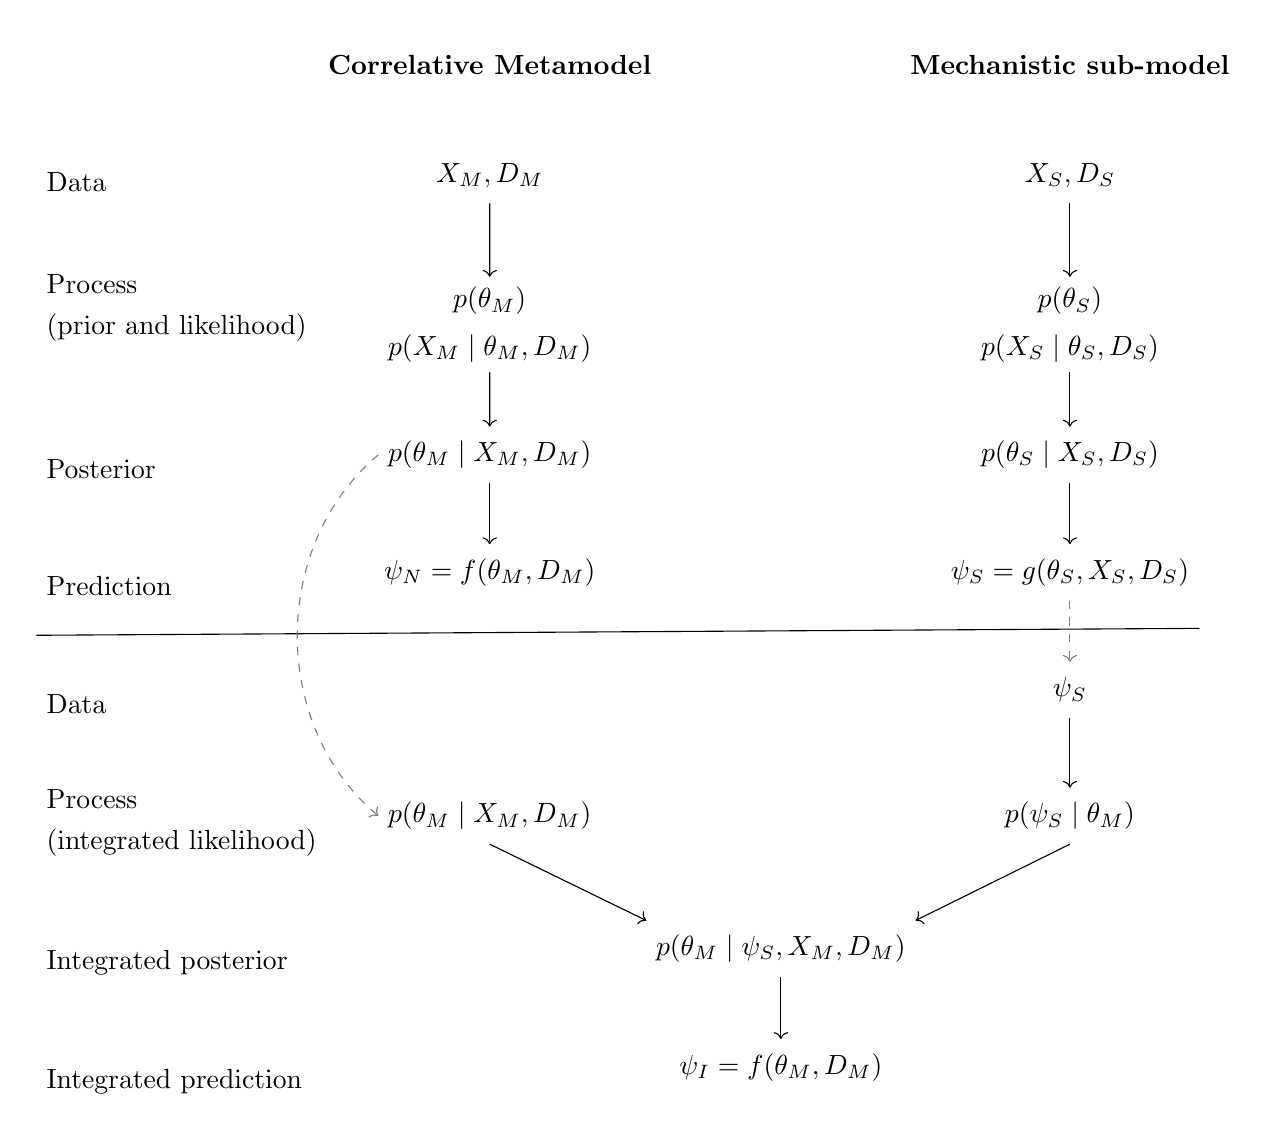
\begin{tikzpicture}
	
\matrix(m) [matrix of nodes, column sep=-0.5em,
	row sep=2em,
	minimum width=4em,
	minimum height=2em,
	column 1/.style={anchor=west, align=left, text width=10em},
	multi/.style={rectangle split,rectangle split parts=2}]
	{
	% zeroth line
	% blank space 
	&
	\textbf{Correlative Metamodel}
	&
	&
	\textbf{Mechanistic sub-model}
	\\
	% first line
	Data % m 1-1
	&
	$X_{M}, D_{M}$ % m 1-2
	&
	&
	$X_{S}, D_{S}$ % m 1-4
	\\
%second line
	|[multi]| Process % m 2-1 
	\nodepart{second}
	(prior and likelihood)
	&
	|[multi]|$p(\theta_{M})$ % m 2-2
	\nodepart{second}
	$p(X_{M} \mid \theta_{M}, D_{M})$
	&
	&
	|[multi]|$p(\theta_{S})$
	\nodepart{second}
	$p(X_{S} \mid \theta_{S}, D_{S})$
	\\

%third line
	
	Posterior
	&
	$p(\theta_{M} \mid X_{M}, D_{M})$
	&
	&
	$p(\theta_{S} \mid X_{S}, D_{S})$
	\\

%fourth line
	Prediction
	&
	$\psi_N = f(\theta_M, D_M)$
	&
	&
	$\psi_S = g(\theta_S, X_S, D_S)$
	\\

%fifth line
	Data
	&
	&
	&
	$\psi_S$
	\\
%sixth line
	|[multi]| Process
	\nodepart{second}
	(integrated likelihood)
	&
	$p(\theta_M \mid X_M, D_M)$
	&
	&
	$p(\psi_S \mid \theta_M)$
	\\


%seventh line
	Integrated posterior
	&
	&
	$p(\theta_M \mid \psi_S, X_M, D_M)$
	&
	\\

%eighth line
	Integrated prediction
	&
	&
	$\psi_I = f(\theta_M, D_M)$
	&
	\\
}; %end matrix

% The names of the nodes are automatically generated in the previous matrix. Since the
% matrix was named ``m'', all nodes have the name m-row-column

% metamodel
\draw [->] (m-2-2.south) -- (m-3-2.north);
\draw [->] (m-3-2.south) -- (m-4-2.north);
\draw [->] (m-4-2.south) -- (m-5-2.north);

%%mechanistic model
\draw [->] (m-2-4.south) -- (m-3-4.north);
\draw [->] (m-3-4.south) -- (m-4-4.north);
\draw [->] (m-4-4.south) -- (m-5-4.north);

%%separation line
\draw [line cap=rect, transform canvas={yshift=-1em}] (m-5-1.south west) -- (m-5-4.south east);
%(\linewidth-\pgflinewidth,0); 

\tikzstyle{opt}=[gray,dashed,rounded corners];
\draw [->,style=opt] (m-4-2.west) to[bend right=50] (m-7-2.west);
\draw [->,style=opt] (m-5-4.south) to (m-6-4.north);

%%integrated model
\draw [->] (m-7-2.south) -- (m-8-3.north west);
\draw [->] (m-6-4.south) -- (m-7-4.north);
\draw [->] (m-7-4.south) -- (m-8-3.north east);
\draw [->] (m-8-3.south) -- (m-9-3.north);


\end{tikzpicture}


\caption{The parameters of a correlative metamodel model (left column) are conditioned on the predictions of a mechanistic sub-model (right column).
	The metamodel ($\theta_M$) operates at a single scale and uses occurrence data (\(X_M\)) and explanatory variables ($D_M$) to produce a naive (i.e., not conditioned on sub-models) prediction $\psi_N$.
	The mechanistic sub-model \(\theta_S\) includes data about the response (\(X_S\)) of lower-level behaviours of the system to explanatory variables ($D_S$). 
	The models are integrated by calibrating $\theta_M$ to data ($X_M, D_M$) as well as the output of the sub-model ($\psi_S$). 
	This is possible because predictions from the sub-model ($\psi_S$) emerge at the scale of the metamodel via a scaling function \(g(\theta_S, D_S)\).
	This prediction incorporates multiple sources of information coming from several calibration datasets (i.e., $X_M, D_M, X_S, $ and $D_S$) as well as from multiple types of models (i.e., $\theta_M$ and $\theta_S$).}
\label{fig:diagram}
\end{figure}
%==================

Using Bayes' theorem, we find the posterior probability of \(\theta_M\) as follows:
%-----
\begin{equation}
\label{eq:sdm3}
	p( \theta_M \mid X_M, D_M ) = \frac{ p( X_M \mid \theta_M, D_M ) p( \theta_M ) } { p(X_M, D_M) }
\end{equation}
%-----
where \(p( X_M \mid \theta_M, D_M )\) is referred to as the likelihood of the observations, \(p(\theta_M )\) is the prior probability of the model, and \(p(X_M, D_M)\) is the normalization constant.
The normalization constant involves computing integrals that are often impossible to solve analytically. 
In practice, simulation techniques such as MCMC can be used to sample directly from the posterior distribution, making such computations unnecessary \citep{Link2006}.
Thus, we use the proportional form of Bayes' Theorem:
%-----
\begin{equation}
\label{eq:sdm4}
	p( \theta_M \mid X_M, D_M ) \propto p( X_M \mid \theta_M, D_M ) p( \theta_M ) 
\end{equation}
%-----

The role of the metamodel is to integrate data at the same ecological scale of predictions.
Additional sub-models require outputs that should be comparable to this given ecological scale (e.g. constraining presence or absence on the landscape).
Formally, we will add an additional model, \(\theta_S\), that is based on a different set of hypotheses and that makes predictions \((\psi_S)\) based on an additional dataset \((X_S, D_S)\):
%-----
\begin{equation}
\label{eq:model2-1}
	\psi_S = g(\theta_S, X_S, D_S)
\end{equation}
%-----

For integration to be successful, it must be possible to compute the likelihood of this prediction given the metamodel, \(p \left( \psi_S \mid \theta_M \right) = p \left(\theta_S \mid \theta_M, X_S, D_S \right)\); the function \(g\) serves to transform the parameters of the sub-model to the scale of the metamodel. Thus, we refer to \(g\) as the \emph{scaling function}. 
In many cases, computing this likelihood will be challenging.
The simplest case is when the parameters of \(\theta_S\) are directly comparable to those in \(\theta_M\), or when the scaling is performed directly within the sub-model, but other solutions are possible.
This new likelihood, which integrates the information from the second model into the first, can be treated as new ``data'' to evaluate the parameters of \(\theta_M\).
We simply use the posterior distribution of \(\theta_M\) from the previous step (Eq. \ref{eq:sdm4}) as the new prior probability of \(\theta_M\), and evaluate the posterior probability of \(\theta_M\) in light of the new data (i.e., information from the submodel \(\theta_S\)) and the prior knowledge, as before:

%-----
\begin{equation}
\label{eq:integrated2}
	\overbrace{p( \theta_M \mid X_M, D_M, \theta_S, X_S, D_S )}^\text{integrated posterior}
	\propto 
	\overbrace{p( \theta_S \mid \theta_M, X_S, D_S )}^\text{likelihood}
	\overbrace{p( X_M \mid D_M, \theta_M ) P( \theta_M )}^{\text{prior for } \theta_M}
	\overbrace{p(\theta_S)}^{\text{prior for } \theta_S}
\end{equation}
%-----

This procedure may be applied to an arbitrary number of models, limited only by available data and computational power. 
The models may be implemented simultaneously, when multiple datasets are available and can be evaluated under different underlying models, or they may be run sequentially, updating the posterior distribution of \(\theta_M\) as new information becomes available. 
Note that \(\theta_S\) itself need not be implemented in a Bayesian framework and the output need not be identical in form to the output of \(\theta_M\); it is enough to produce an output that can be evaluated as a likelihood under the first model and to have some assessment of the confidence in the parameter estimates of \(\theta_S\) to use as a prior.

%---------------------------------------------
%---------------------------------------------

\section*{Example 1}
To produce the simulated dataset used in the first example, we first simulated 100 presence-absence points at randomized locations in ecological space (i.e., temperature and precipitation) using the spsample function from package sp in R \citep{Bivand2013, R}.
This function generates points with a specified amount of spatial clustering (ranging from 0 to 1, where 1 represents complete spatial independence); we selected a value of 0.2 for our analysis.
Presence or absence at each point was determined by randomly sampling from a Bernoulli distribution, where the probability was selected using a pre-determined function of temperature and precipitation.
We then fit the naive model in JAGS as a logistic regression, with both linear and quadratic terms for both temperature and precipitation and using uninformative priors (Normal with \(\mu = 0\) and \(\sigma = 10000\)).
We discarded the first 5000 MCMC samples as burnin, and then collected an additional 2000 samples for analysis.
The final sample size was selected to provide for relatively rapid computational time; the addition of longer final samples or extended burnin periods had no effect on the results.

For the mechanistic submodel, we computed the predicted probability of presence as a function of precipitation, using the experimental data and the theoretical prediction that the species will be present when the population growth rate is greater than 0.
For each of the five experimental treatments, we computed the probability of presence as the integral of the normal density from 0 to infinity, where the mean of the normal distribution was equal to the average population growth rate at each precipitation treatment and the standard deviation was the corresponding standard error for each treatment.
We then fit these data to the same model, priors, and sample sizes as those from the previous step.
Fitting the metamodel is simply a matter of repeating the exact procedure for fitting the naive model, but using informative priors generated from the naive model step.
Because the sub-model considered only precipitation, and because the response was highly correlated to precipitation, we expected the submodel to produce highly precise estimates of the parameters for the effect of precipitation on the probability of presence.
However, the sub-model was quite simplistic, and thus likely over-estimates its precision when considering the species range wholistically (as is done with the metamodel).
Thus, we applied a prior weight of 0.05 to the sub-model.
This allowed the sub-model to inform the integrated model without dominating the results.

All scripts were prepared in R and tested under R version 3.0.3.
The MCMC analyses were performed using the JAGS (Just Another Gibbs Sampler) software package, version 3.4.0 \citep{RJAGS}.
Additionally, the rjags, coda, and sp packages are required to complete the analysis.

\section*{Example 2}
We formulated a metamodel for the second example that allowed for the full use of three sources of data: occurrences from forestry plots (see below) as well as coarser-scale presence-absence information and Phenofit projections \citep[both from][]{Morin2009}.
Plot data originated from four forest permanent plot databases and included samples widely distributed in Eastern North America, from Florida to north Canada (Fig. S\ref{fig:plotmap}).
In the US, we included 86,000 plots standardized since 1990 and monitored until 2013 with up to 4 remeasurements by forest plot \citep{OConnell2013}.
Quebec data were provided from the Ministère des Forêts de la Faune et des Parcs with 12,409 permanent plots, and DOMTAR, a forest company in paper production with 1,741 plots, and surveyed from 1960--2011 with up to 10 remeasurements \citep{MFFP2013}.
Ontario and New-Brunswick included 1,038 and 2,748 plots respectively \citep{Porter1999, Ontario2014}.
Ontario monitored forest plots from 1992--2006 with up to 3 remeasurement, and New-Brunswick from 1985--2010 with up to 7 remeasurements.

\begin{figure}[t]
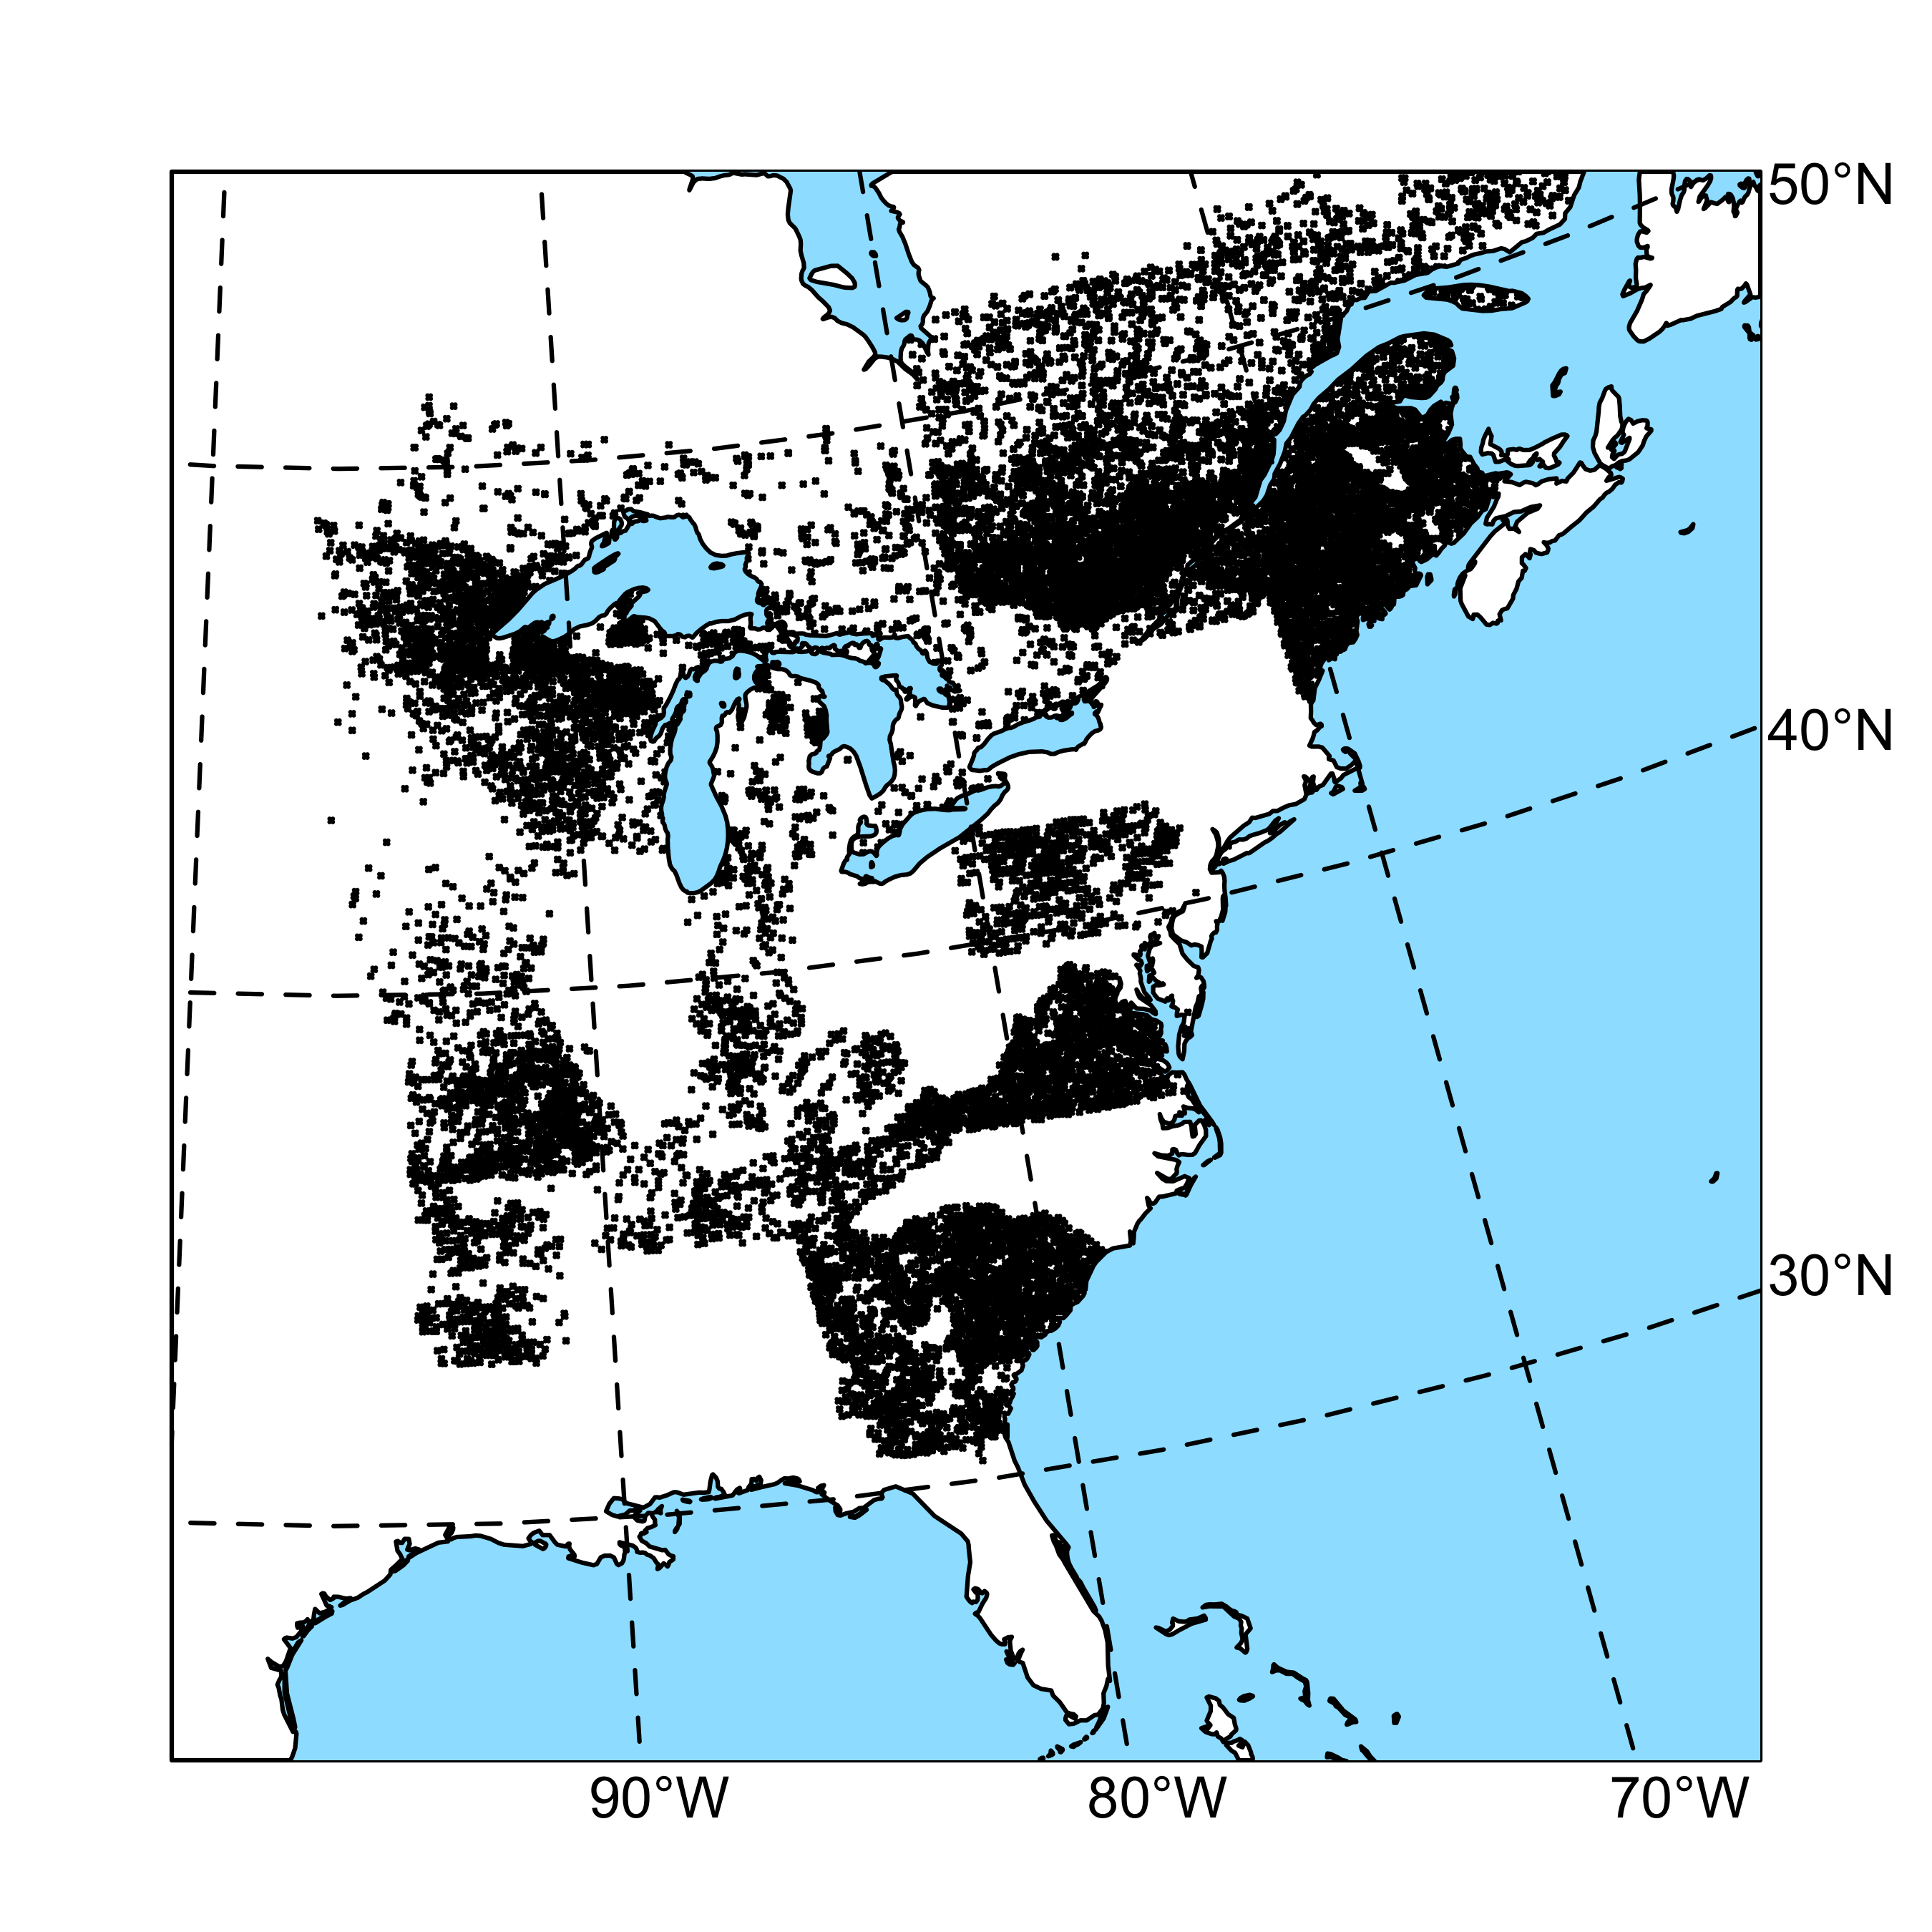
\includegraphics[width=4.5in]{figs/plotmap.png}
\caption{Map of permanent forest plot locations}
\label{fig:plotmap}
\end{figure}

We divided the dataset into calibration and validation subsets, with 1/3 of the data reserved for validation and the remaining 2/3 used for calibration.
As in the previous example, we modeled the probability of presence as a function of climate.
We considered seven climate variables: the number of degree days (ddeg), minimum temperature (min\_temp), potential evapotranspiration (PET), annual precipitation (an\_prcp), summer precipitation (sum\_prcp), winter precipitation (win\_prcp), and the ratio of annual precipitation to potential evapotranspiration (pToPET).
See \citet{Morin2009} for a complete description of these variables.
For projection, we used predictions for \rev{2100} from the HadCM3 GCM \citep{Pope2000} driven by the A2 emission scenario \citep{Nakicenovic2000}, and used the parameters of the models to forecast suitability into the future.
Exploratory analysis revealed that there were collinearities within the predictor variables.
Thus, we only included three variables in the model: ddeg, an\_prcp, and pToPET.
To select the form of the naive model (and thus the metamodel), we used stepwise regression with BIC as the evaluation criteria.
The search scope included all models with linear, quadratic, and cubic terms for all three variables.
\rev{Thus, the naive model (which also defined the scope of the metamodel), can be formulated as a simple Binomial GLM, as in Example 1:
\begin{equation}
\psi_N =\text{logit}^{-1}\left( \theta_M D_M \right)
\end{equation}
where \(\psi_N\) is the probability of presence in the naive model, \(\theta_M\) is the parameter vector of the metamodel (presently unconstrained by any additional information), and \(D_M\) is the macroclimate covariate matrix at the metamodel scale.
The parameter vector is estimated following equation 2 in the main text:
\begin{equation}
p\left (\theta_M \mid X_M,D_M \right ) \propto 
p \left(X_M \mid \theta_M, D_M \right)
p \left(\theta_M \right)
\end{equation}

Because Phenofit provided predictions in the form of a probability of presence (rather than directly in terms of the metamodel parameters as in the previous example), it was necessary to relate these predictions to the metamodel.
We opted to do this via simulation because it is a natural method to use in an MCMC scheme.
We thus treated the Phenofit predictions (\(\psi_P\)) as an observed result of a true underlying set of occurrences (\(X_P\)).
Because these occurrences were unobserved (and in the case of the future distribution, unobservable), it was necessary to infer them using MCMC.
For each MCMC iteration, we generated a simulated occurrence dataset \(\hat{X}_P\) by drawing from a Binomial distribution with probabilities equal to \(\psi_P\).
In order to give both the occurrence dataset and Phenofit predictions equal weight, we drew the same number of samples as were present in the occurrence dataset.
The metamodel was then fit to these simulated data (with conditioning on the naive model as well):
\begin{equation} 
\overbrace{p(\theta_M \mid X_M, D_M, X_P, \psi_P)}^\text{integrated posterior}
\propto
\overbrace{p\left (X_P \mid \theta_M,D_M,\psi_P \right )}^{\substack{\text{new information} \\ \text{from Phenofit}}}
\overbrace{p \left(X_M \mid \theta_M, D_M \right) p \left(\theta_M \right)}^{\substack{\text{naive metamodel} \\ \text{posterior}}}
\overbrace{p \left(\psi_P \right)}^{\substack{\text{prior for} \\ \text{Phenofit}}}	
\end{equation}
This procedure, by generating a random dataset with each iteration, incorporated the variance in the Phenofit predictions.
Finally, because we were interested in two separate questions with respect to Phenofit integration (one regarding how integration affects uncertainty in our present estimate of the species distribution and a one regarding the effect of integration on projections into the future), we performed two separate integrations with the Phenofit information.
To address the first question, we used the Phenofit predictions for the present as \(\psi_P\) and present climate as \(D_M\), producing the Integrated-Present model.
To address the second, we used the future predictions from Phenofit and future climate, resulting in the Integrated-Future model.
In both cases, the naive model was a GLM relating present occurrences to present climate (and thus the prior response to the environment was static, similarly to how one might use the same conventional SDM to both model present distribution and project into the future).
Convergence for all models was assessed by comparing the results of multiple chains with overdispersed starting points.
Based on the results of these initial runs, we thinned all posterior samples by recording only every 50th sample, and we obtained 25000 posterior samples for each model following a burn-in period of 20000 samples.}

\section*{Implementation}
\rev{Here, we provide a brief guide on implementing our framework. We focus on our two examples, providing a brief outline of the steps to reproduce the analyses using the code and data provided in Appendix S2.
In the section for each example, we provide some references to software packages that may be of assistance to beginning users.
As a full discussion of the practicalities of Bayesian modelling is beyond the scope of this paper, we direct the reader to some of the many excellent resources for Bayesian and hierarchical modelling in ecology \citep[e.g., we suggest][]{Bolker2007, Royle2009, Link2010}.
We also provide some additional information on applying model weights.
Our intent is that, with this guide and the accompanying code, users familiar with R and with some experience with Bayesian modelling will be able to implement our method.}

\subsection*{Example 1}
\rev{
Example 1 is implemented fully using off-the shelf statistical software.
Data preparation, exploration, and visualization is all performed in R \citep{R}.
Parameterization of all models is performed using JAGS, which is a standalone implementation of a Metropolis-Hastings and Gibbs sampler, as well as RJAGS, the R interface to the JAGS program \citep{RJAGS}.
Within the {\tt example\_1} directory in Appendix S2, we provide 6 numbered scripts.
These are designed to be run from the command line using the RScript program that ships with most standard R installations (e.g., {\tt Rscript 1-m1.r} to run the first script).
However, we encourage users to review the code rather than simply running the examples from the command line.
Users of the R console (or the RStudio environment) will be able to run the code one line at a time, provided the working directory is set to the {\tt example\_1} directory beforehand.

There are three main steps to running the analysis, corresponding to the first three numbered scripts.
The first (file {\tt 1-m1.r}) generates the simulated presence-absence dataset, loads a JAGS model representing the metamodel (from the file {\tt ex1\_metamodel.jags}), and runs JAGS on the model to produce posterior samples for the naive model.
Note that, because the naive model and the metamodel are at the same scale and differ only in whether they include additional information from the sub-model, the JAGS model file is the same for both.
All data and results from this step are saved to the {\tt dat/ex1\_m1.rdata} file.
Step two ({\tt 2-m2.r}) creates the dataset for the sub-model, loads the JAGS model ({\tt ex1\_model2.jags}), and runs the model, saving all results to {\tt dat/ex1\_m2.rdata}.
Finally, the third step ({\tt 3-mm.r}) simply reads the estimates from the sub-model, incorporates them into the information passed to JAGS for estimating the metamodel, and runs JAGS to obtain the integrated posterior samples and save them to {\tt dat/ex1\_mm.rdata}.
The posterior samples are saved as MCMC objects from package coda; users should refer to the documentation for that package for information on using these objects.
The remaining three scripts contain code for reproducing the figures contained in the main manuscript.
Users may find them useful for guidance on working with posterior samples generated with JAGS.
}


\subsection*{Example 2}
\rev{
For performance reasons, we have implemented Example 2 as a standalone C++ program, designed to be run multi-threaded in high-performance computing applications.
Due to the size of the dataset and the increased complexity of the model (relative to Example 1), the computational load is considerably higher.
The procedure to compile and run the model is also somewhat more complex.
Therefore, to facilitate exploration without requiring users to actually build and run the model, we have included the posterior samples we obtained with Appendix S2.
This will allow users to build the figures and explore the results of the naive and integrated models.
For the portions that can be run in R, as in Example 1, we have included numbered scripts that can be run with {\tt Rscript}.
There are three scripts included in the {\tt example\_2/r/} directory, numbered 1, 3, and 5 (steps 2 and 4 are running the C++ program to obtain samples for the naive and integrated models, respectively).
Step 1 ({\tt 1\_prepare\_naive\_data.r}) prepares the dataset for the naive model to be used with the sampler, resulting in the files {\tt dat/mcmc/naiveData.csv} (for use with the C++ program) and {\tt dat/mcmc/naiveData.rds} (for use with R, can be loaded using the {\tt readRDS} function).
Step 2 (see following paragraph) creates the file {\tt results/mcmc/naivePosterior.csv}, which contains the posterior samples for the naive model and which we have included for users that do not wish to build and run the C++ program themselves.
Step 3 reads the results of the naive model estimation and uses it to prepare the files needed to estimate the integrated model.
As with step 2, step 4 depends on the C++ program and produces posterior samples for both the Integrated-Present and Integrated-Future models (files {\tt integratedPresent.csv} and {\tt integratedFuture.csv}, respectively, in the {\tt results/mcmc/} directory).
Finally, step 5 reads all of the CSV files containing posterior samples and processes them into MCMC objects (saved in {\tt results/posteriors.rdata}) that can be easily manipulated in R with the coda package.
We also include code for reproducing the figures contained in the manuscript (all scripts starting with {\tt fig}), and a brief interactive script for performing model evaluation ({\tt evaluation.r})

For users wishing to build and run the C++ program to estimate the posterior distributions, some knowledge of C++ compilers will be required.
A familiarity with GNU Make will also be of assistance, because the build procedure is fully automated and documented within the included makefile.
All C++ code is contained within the {\tt src} subdirectory and should be fully compatible with any platform capable of compiling and running standard C++89 programs.
The only external dependency is the GNU Scientific Library (freely available at http://www.gnu.org/software/gsl/), an open-source C library which we have used for random number generation and other mathematical operations.
Additionally, for high-perfomance computing applications, we have included compiler commands for using OpenMP.
When enabled, this will significantly improve the speed at which the likelihood is computed, and thus reducing the runtime of the model.
All compiler commands, as well as the commands used to run the model and generate posterior samples, are included in the makefile.
Additionally, once the program is compiled, help with program options can be obtained using the {\tt -h} switch (i.e., {\tt integrated\_model -h} at the command line).
}
 
\subsection*{Model weights}
\rev{Model weights, expressed mathematically as the prior probability of each individual sub-model, allow the user to express prior belief that a particular sub-model is effective at describing the range of a species.
This is particularly useful, as in Example 1, when a sub-model is highly statistically precise but, due to limited scope, is not effective alone at describing the range of a species.
The hypothetical experiment in Example 1 included only 5 treatments in a single variable, and thus misses many important processes that generate species ranges.
Selecting the specific weighting to use will, of necessity, be somewhat subjective, as it is often difficult to express prior belief of this sort in precise mathematical terms.
As a start, users may consider weighting models based on sample size or number of independent treatments, as we have done in example 1, where the weight for the sub-model of 0.05 was chosen based on the 5 precipitation levels relative to 100 independent data points in the correlative dataset.
Implementation of the weights within the model code itself will depend on the implementation.
In the case of Example 1, the weight was applied by decreasing the precision of all terms that were informed by the submodel (i.e., making the prior that resulted from the sub-model less informative).
}

\renewcommand\refname{Literature Cited}
\bibliography{model_integration}{}
\bibliographystyle{model_integration}

\end{document}